
\begin{figure}
    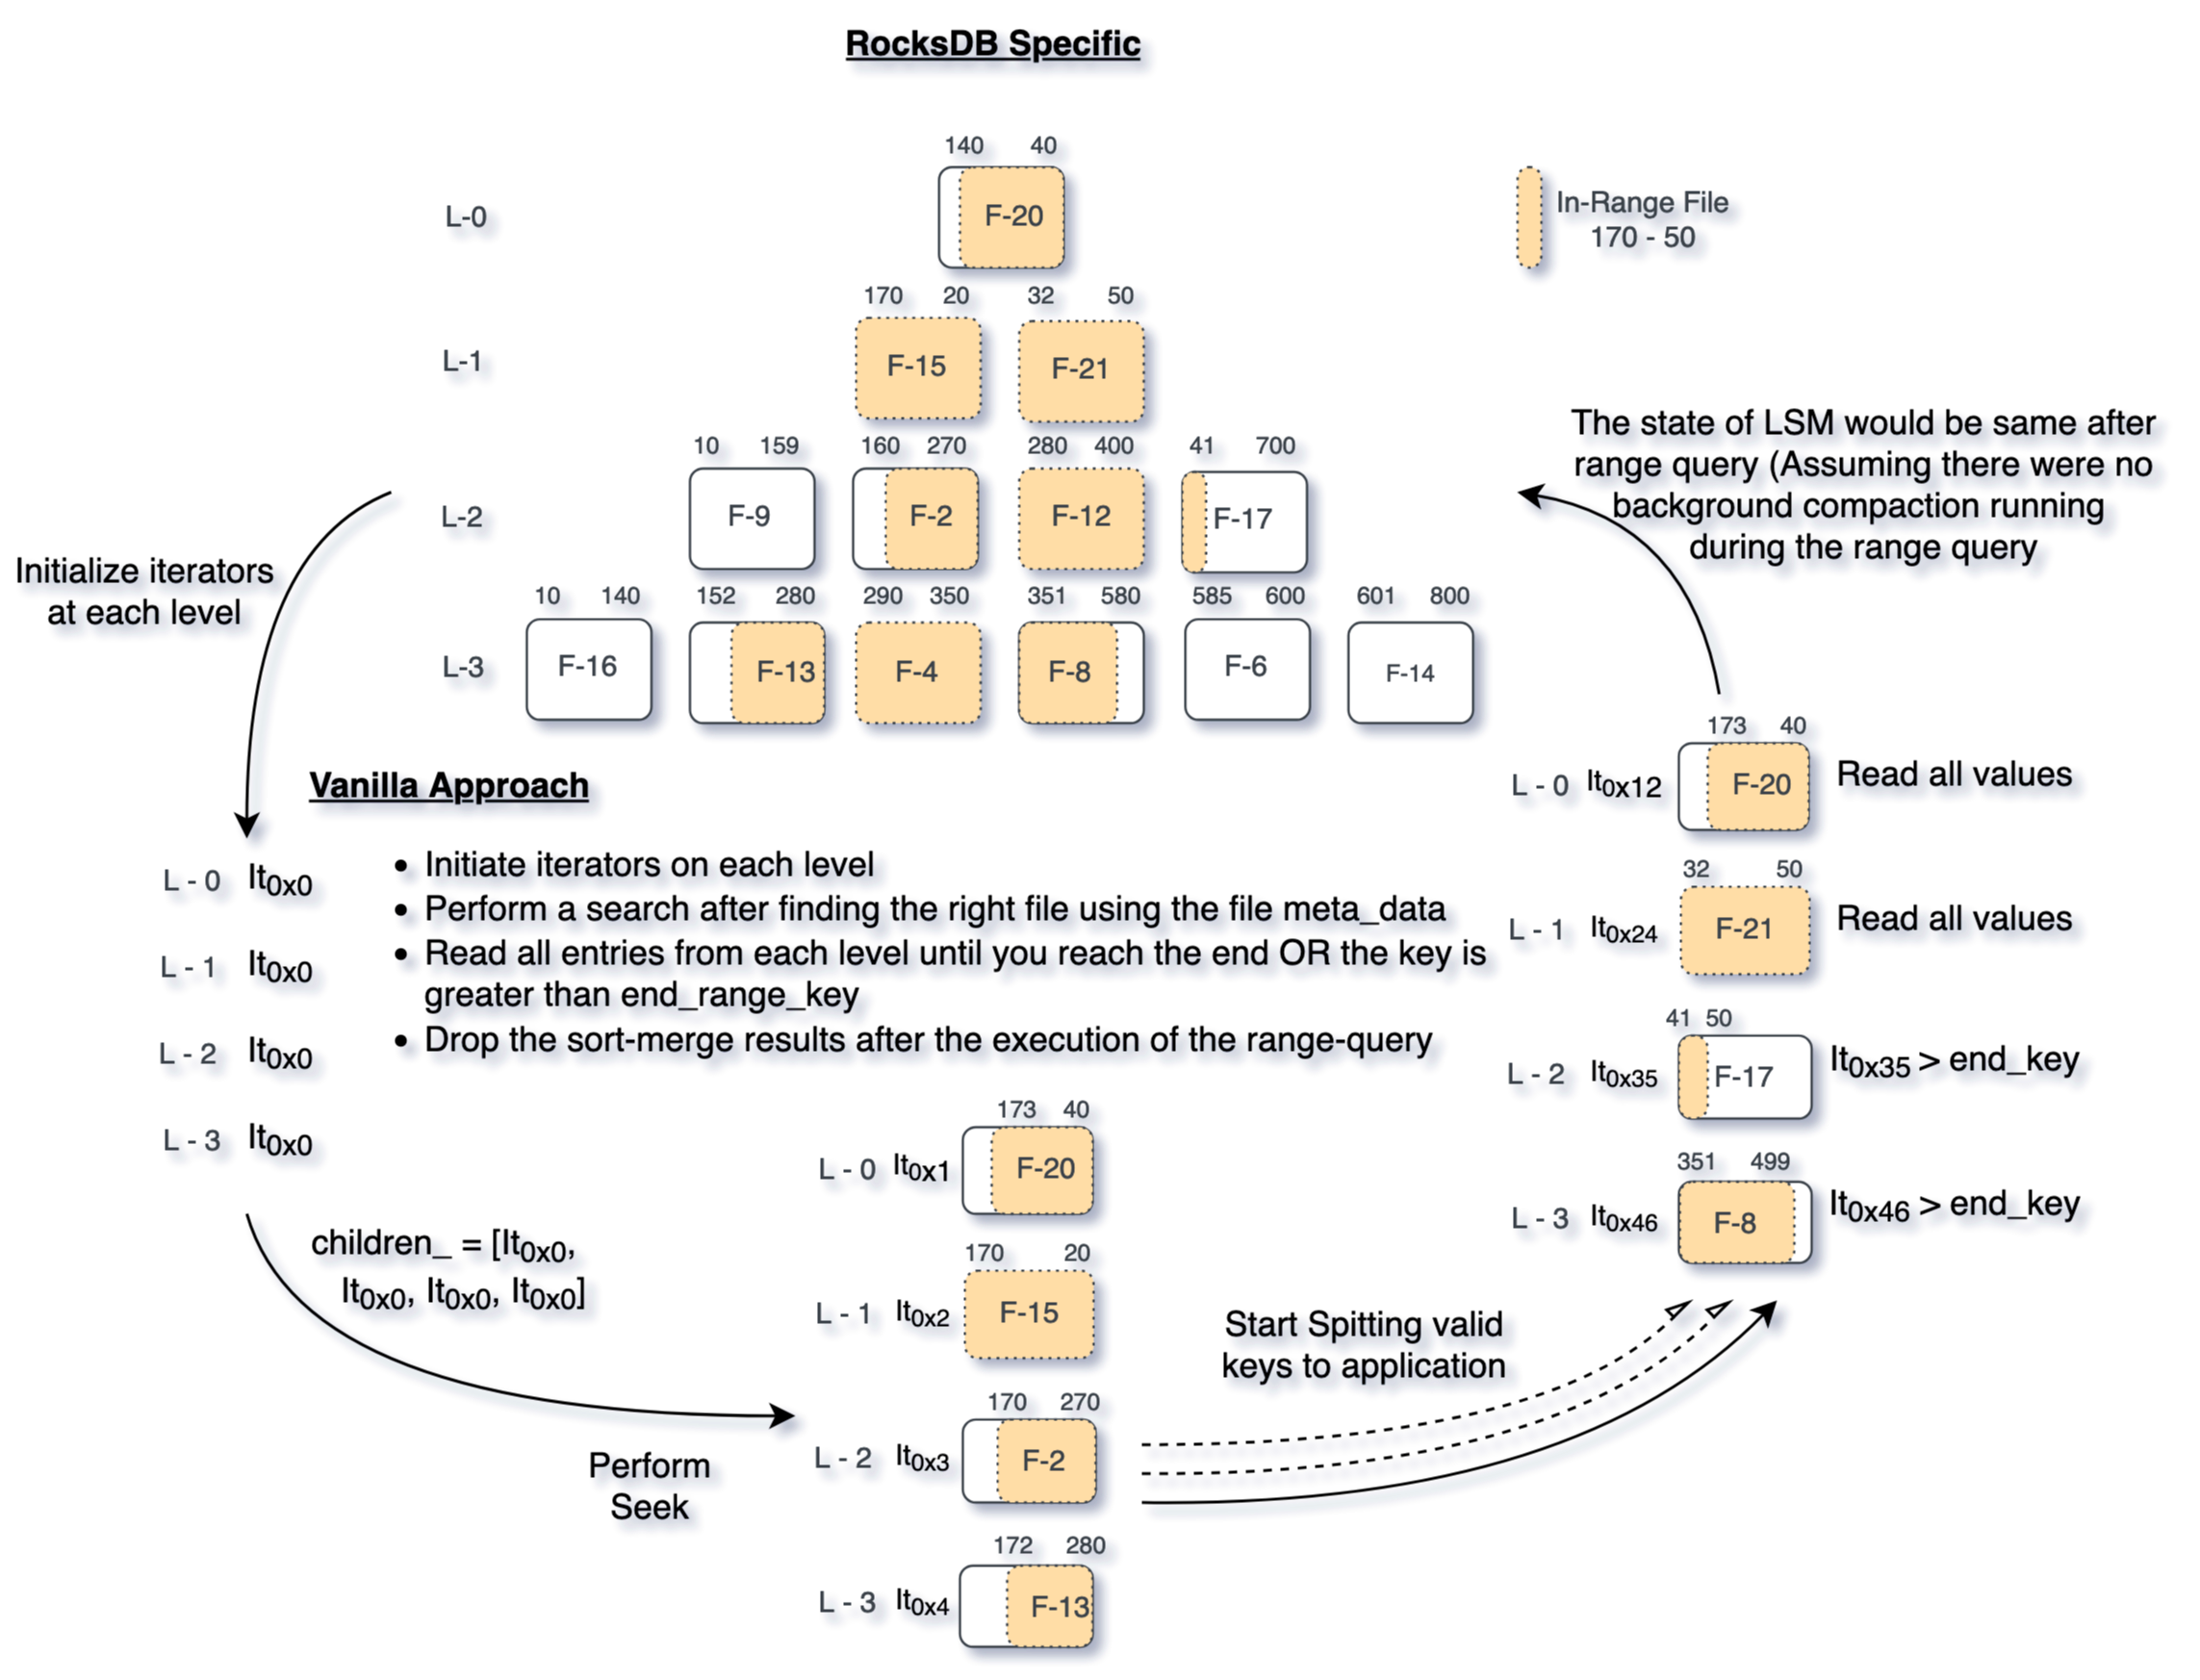
\includegraphics[scale=0.10]{Figures/Vanilla Range Query rocksdb specific.png}
    \caption{Range query flow in lexicographically sorted files}\label{fig:rocksdb_specific_vanilla_range_query}
\end{figure}


\begin{figure*}
    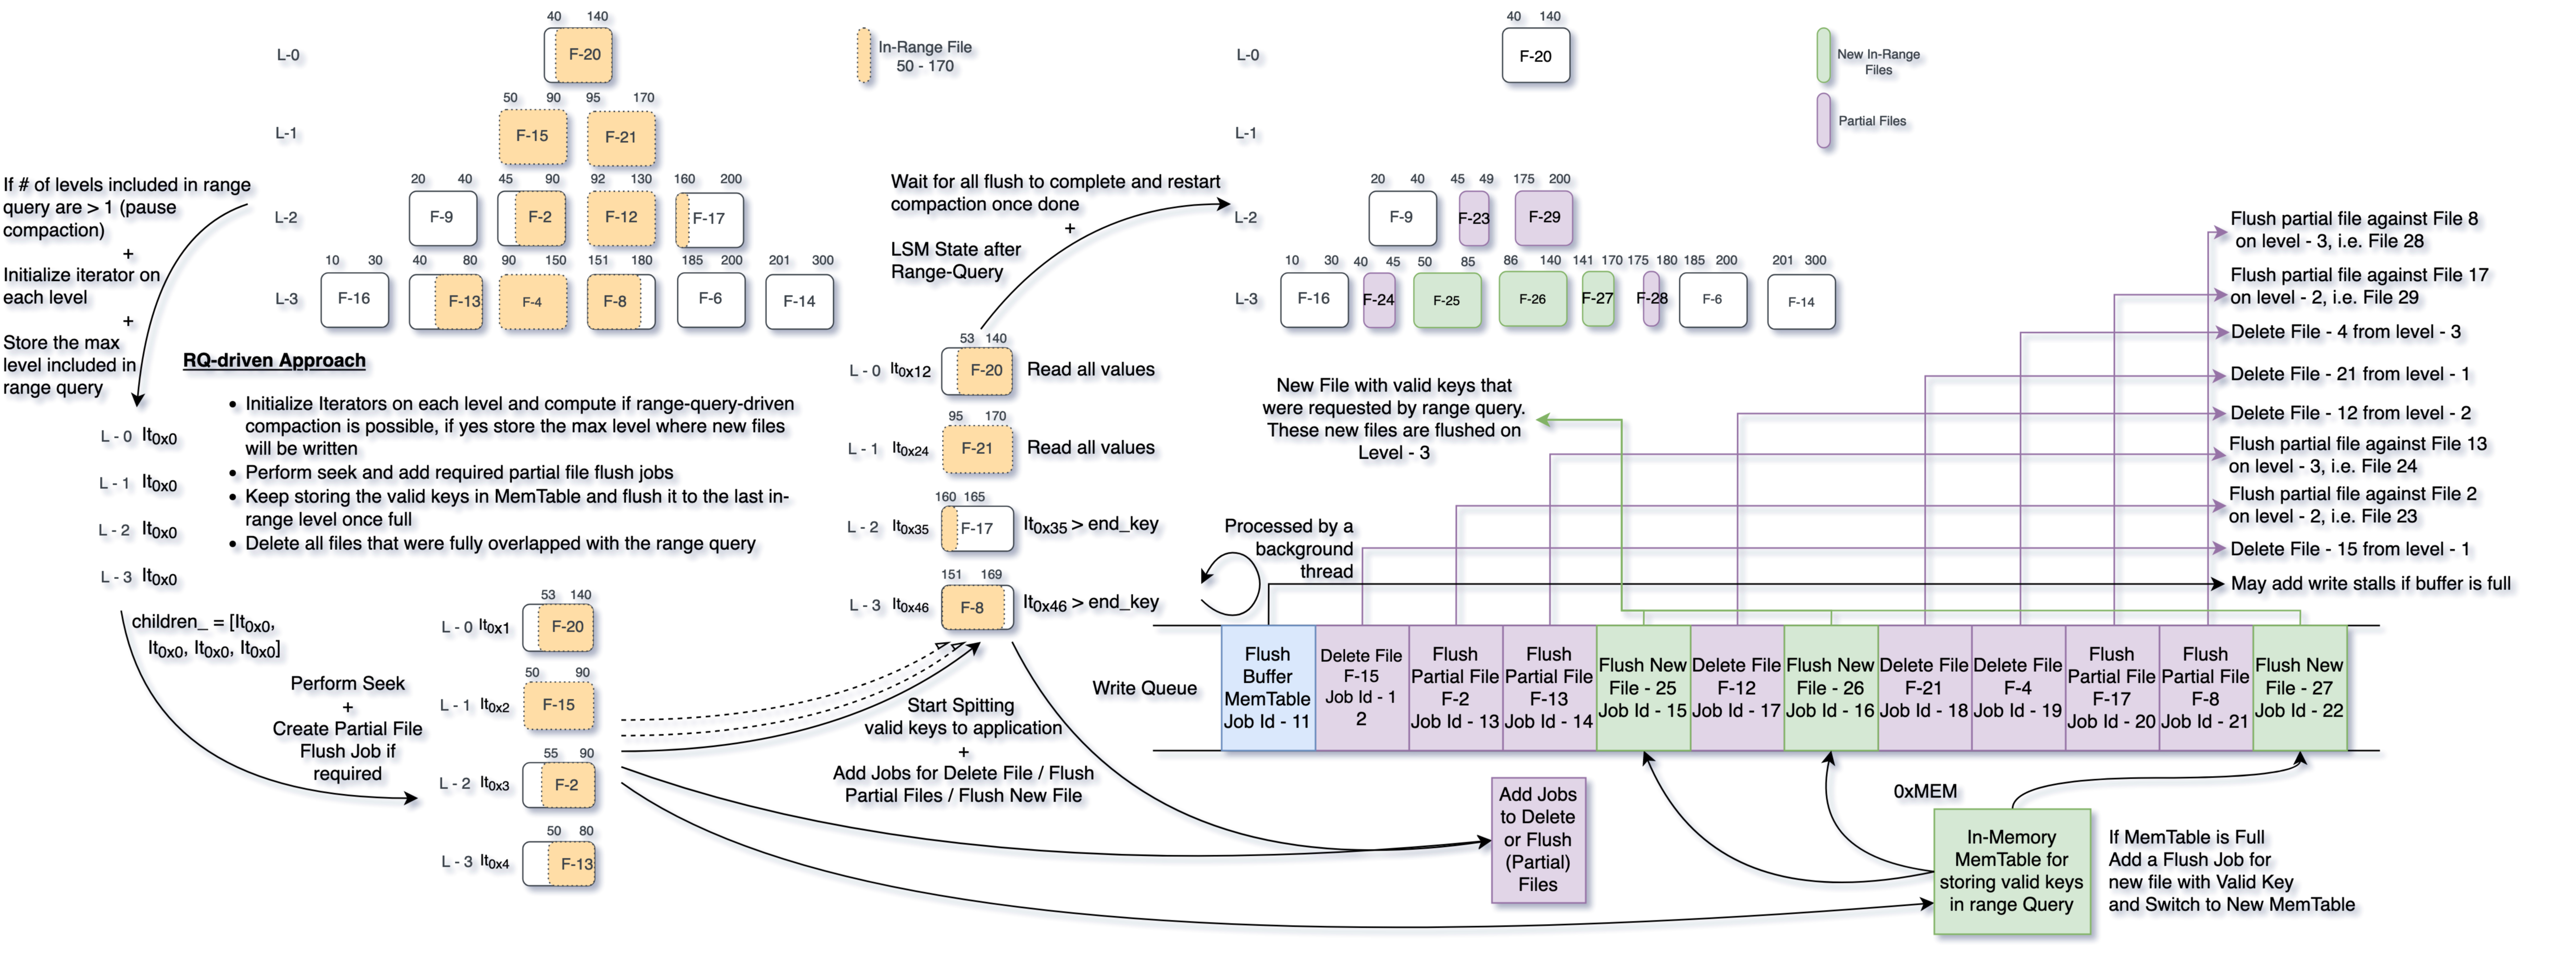
\includegraphics[scale=0.10]{Figures/RQ-driven numeric key sorting.png}
    \caption{Query-driven compaction flow in LSM}\label{fig:query-driven_compaction}
\end{figure*}

\begin{figure}
    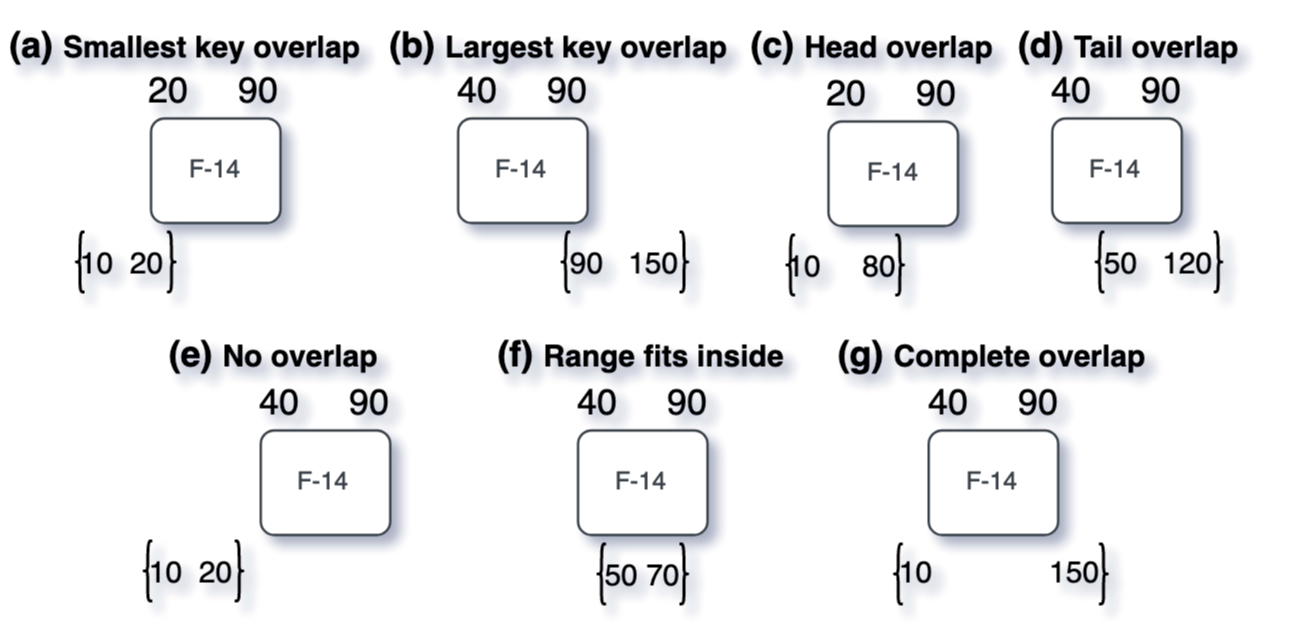
\includegraphics[scale=0.2]{Figures/File range overlaps.png}
    \caption{File range-query overlaps}\label{fig:file_range_overlaps}
\end{figure}

\begin{figure*}
    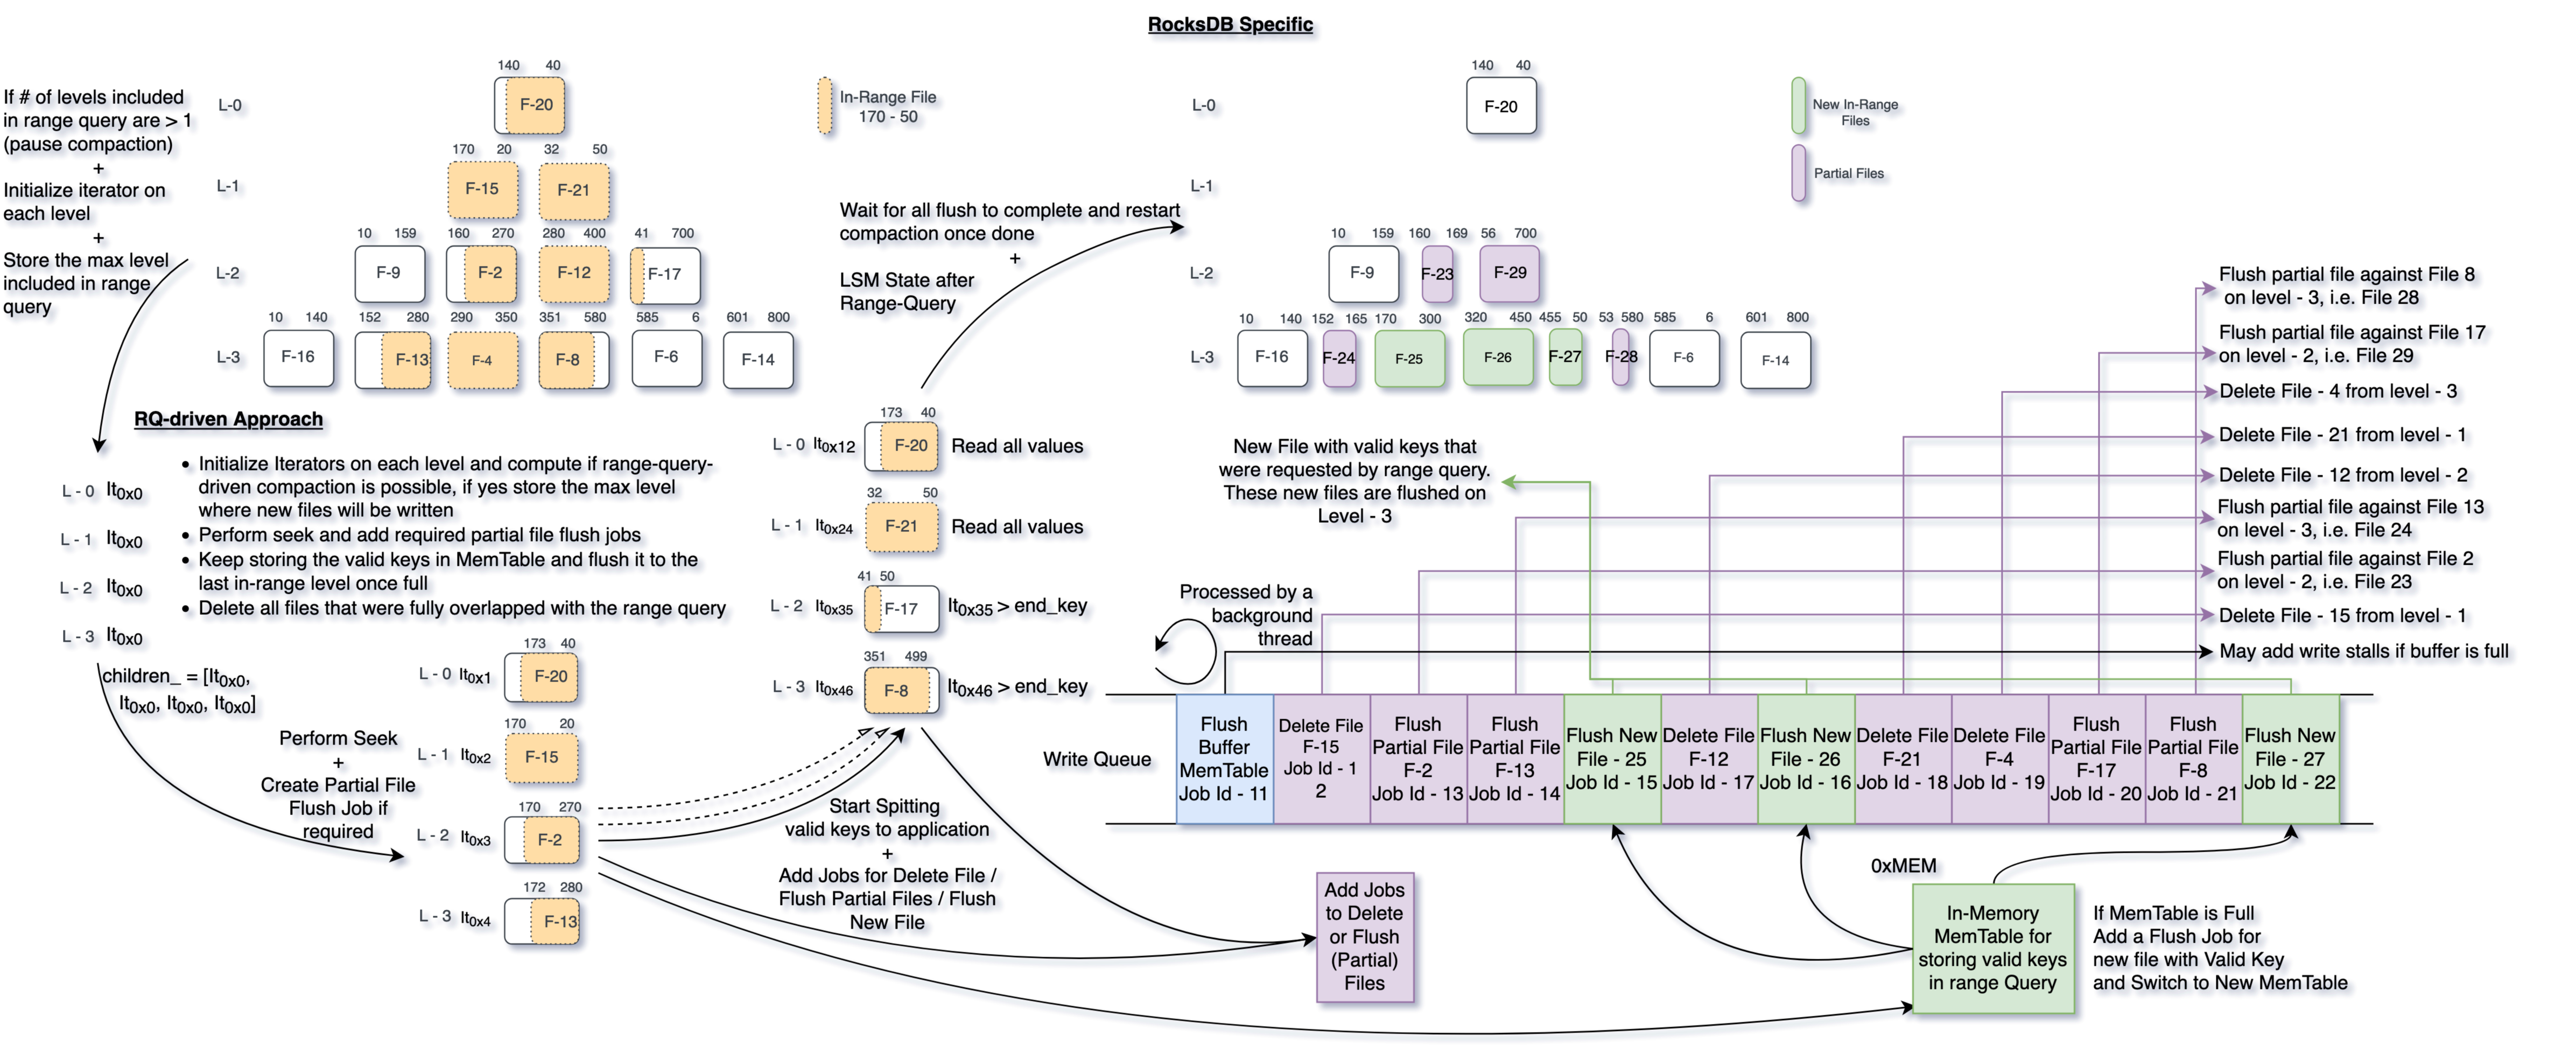
\includegraphics[scale=0.10]{Figures/RQ-driven rocksdb specific.png}
    \caption{Query-driven compaction flow in lexicographically sorted files}\label{fig:rocksdb_specific_query-driven_compaction}
\end{figure*}

The solution to the problem of redundant work and increased write amplification is query-driven compaction. This 
approach involves writing the valid keys back to the higher levels of the LSM tree.

\subsection{Vanilla Approach}
The flow of range query in vanilla approach is shown in Figure-\ref{fig:vanilla_range_query} and 
Figure-\ref{fig:rocksdb_specific_vanilla_range_query}. The query runs by 
initiating the iterators for each level of LSM tree and then perform a seek operation on each iterator to find the 
first key that is greater than or equal to the start key of the range query. It then iterates through the
SSTables in the LSM tree and returns the values that fall within the key range. At the end of the range query
execution the state of LSM tree would be same as before the query execution.

\subsection{Query-driven Compaction}
The flow of range query in query-driven compaction is shown in Figure-\ref{fig:query-driven_compaction} and 
Figure-\ref{fig:rocksdb_specific_query-driven_compaction}. The initial 
setup of level iterators goes the same as in the state-of-the-art LSM range query. Once all the iterators are 
initialized, it performs a seek operation on iterators using the range-query start\_key for each level. The seek 
operation in query-driven compaction performs an extra operation to create a partial file flush job and add it to the 
write\_queue\_. The partial file flush will only happen if the file does not completely overlap with the range-query 
start\_key and end\_key. We can have three scenarios for the partial file flush, which 
(as shown in Figure-\ref{fig:file_range_overlaps}) are as follows.

\begin{figure*}
    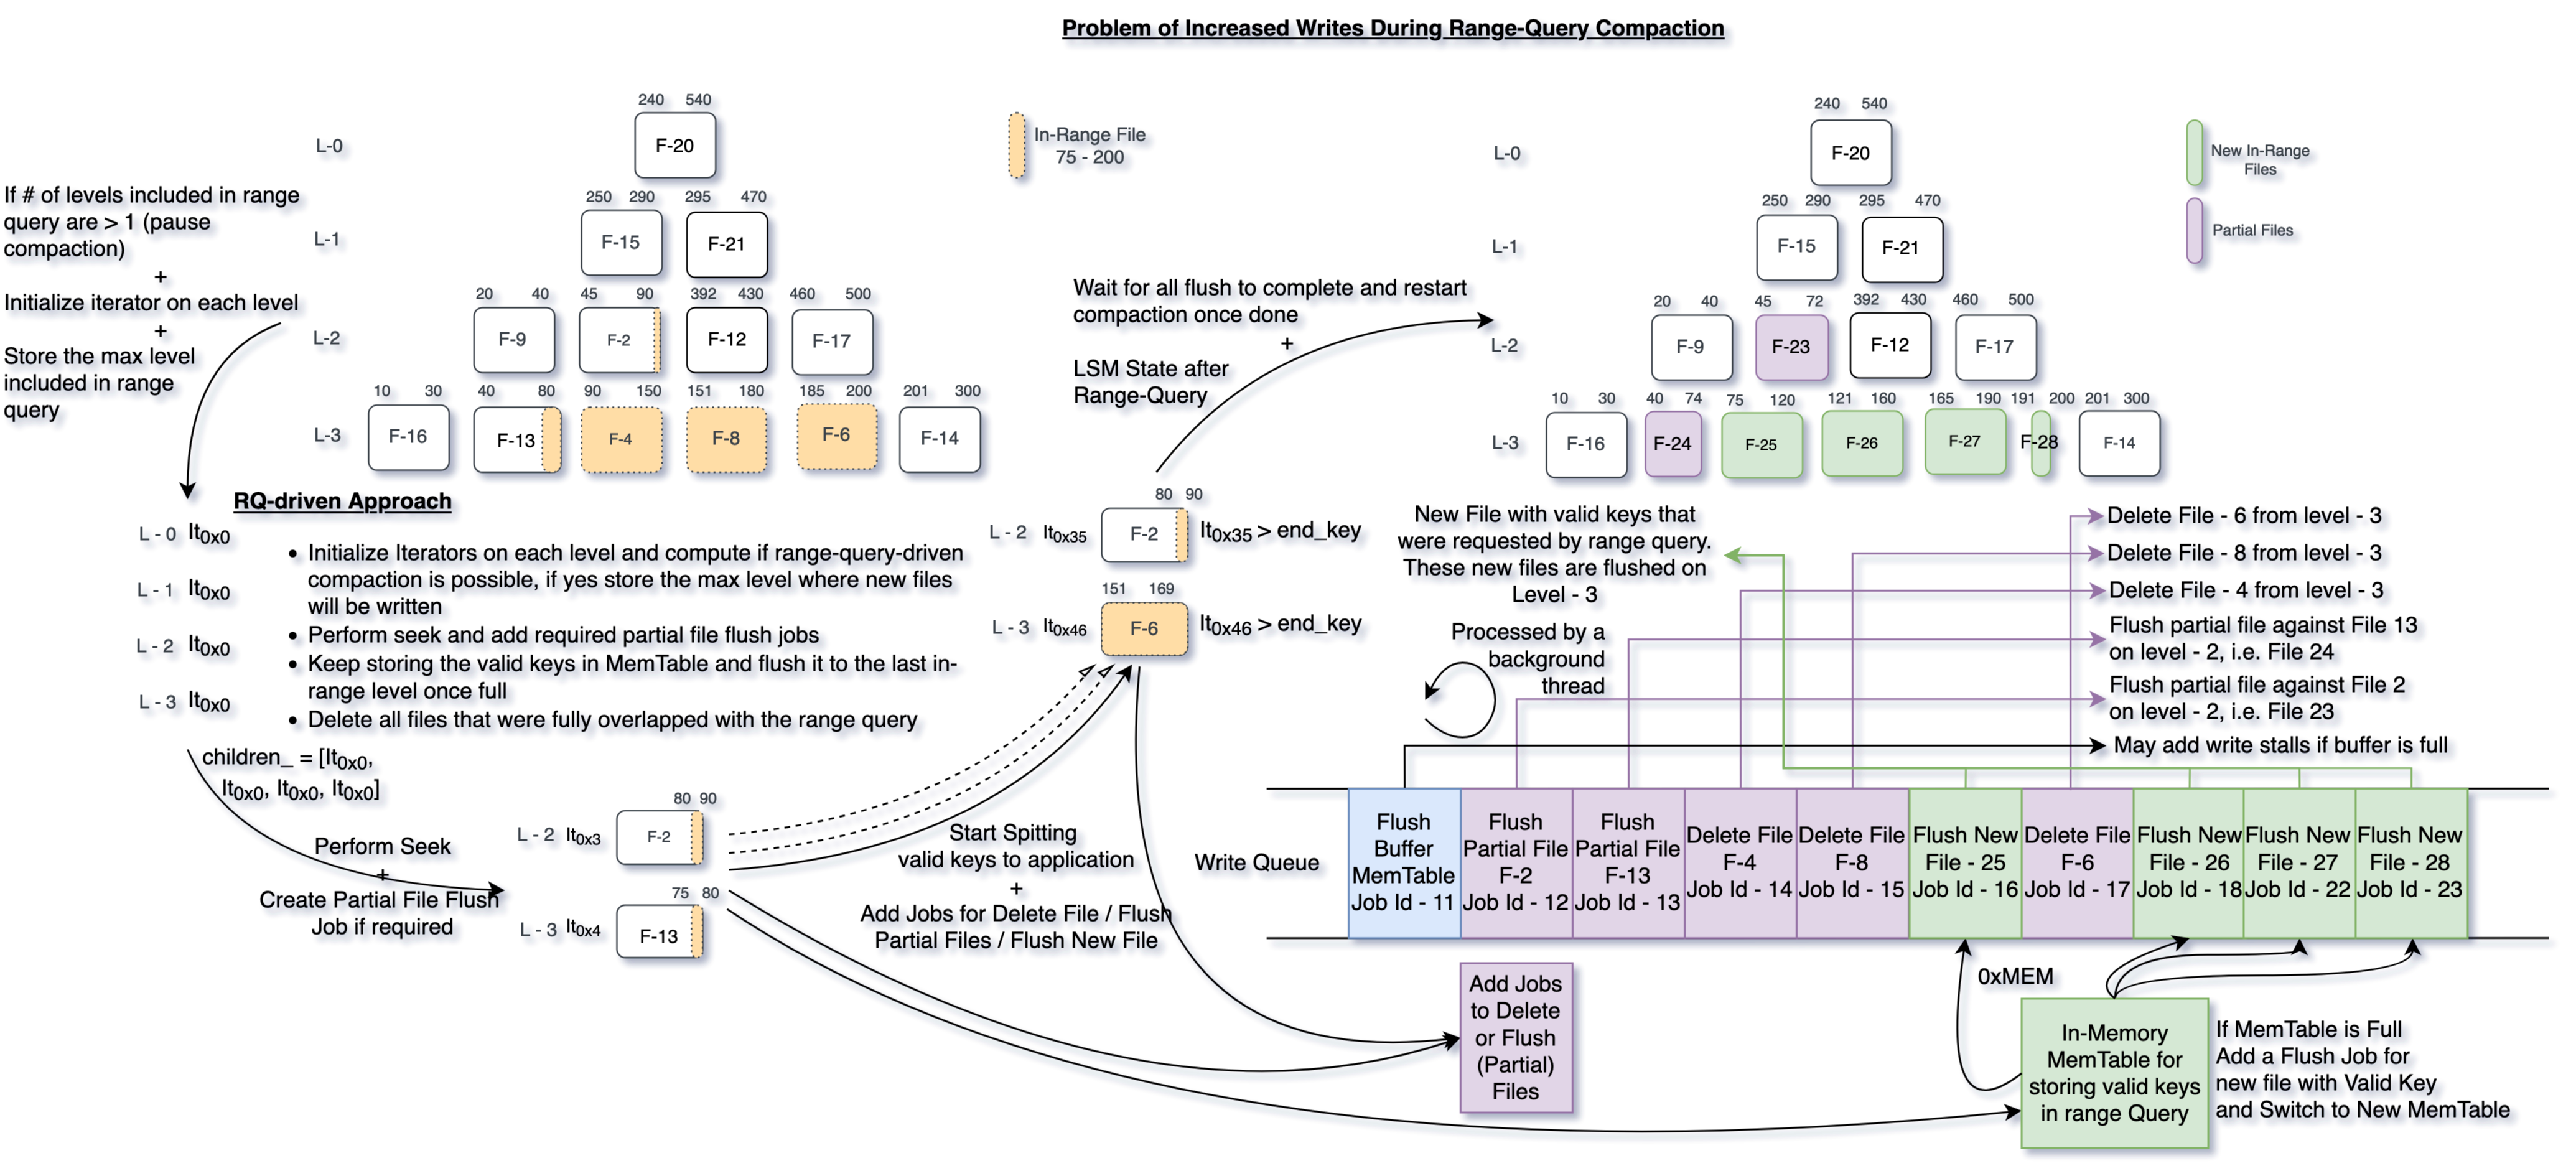
\includegraphics[scale=0.12]{Figures/RQ-driven problem of increased writes.png}
    \caption{Query-driven compaction with increased writes problem due to less overlap}\label{fig:query-driven_compaction_with_increased_writes}
\end{figure*}

\begin{enumerate}
    \item \textbf{No overlap} In this scenario, the partial file flush will not happen as the file does not overlap. 
    Figure-\ref{fig:file_range_overlaps} (e)
    \item \textbf{Smallest or Largest key overlap \textit{(Partial Flush)}} In this, the smallest or largest key of the 
    file overlaps with the range query start or end key. Figure-\ref{fig:file_range_overlaps} (a) and (b)
    \item \textbf{Head or Tail overlap \textit{(Partial Flush)}} In this, the partial part (having more than one key) 
    overlaps with the range query. Figure-\ref{fig:file_range_overlaps} (c) and (d)
    \item \textbf{The range fits inside file overlap \textit{(Partial-Partial Flush)}} Both the start and end keys of 
    the range query fit completely in the file's smallest and largest keys. Figure-\ref{fig:file_range_overlaps} (f)
\end{enumerate}

These partial flush jobs, that are added to the write\_queue\_ are executed by the $Priority::HIGH$ background thread, 
parallel to the range query. It flushes the partial part of the file that does not fall in the range query to the same 
level in the LSM tree.

The files that are completely overlapping with the range query start\_key and end\_key will be deleted from the lower 
levels and the valid keys will be added to the higher levels in new files. We can have one scenario for the file 
deletion from the lower levels which is as follows.

\begin{enumerate}
    \item \textbf{Complete overlap i.e. start\_key <= smallest key and end\_key >= largest key 
    \textit{(Just Delete)}} All files in the lower level, as well as in higher level, that are completely overlapping 
    with the range query will be deleted by the query-driven compaction. Figure-\ref{fig:file_range_overlaps} (g)
\end{enumerate}
The query-driven compaction also initiates an in-memory buffer of the default size configured in db\_options to keep 
copies of the valid keys and flush them back to the LSM when it is full. The main thread, that is executing the range 
query will keep on performing the sort-merge operation and return the valid keys back to the application. Whenever it 
returns a valid key to the application, the query-driven compaction makes a copy and stores it in a memtable. Once the 
memtable is full, it creates a new flush job and adds it to the write\_queue\_. The query-driven compaction also adds 
write stalls for each range query to flush all the jobs initiated during this operation. This happens by stopping the 
background work during the start of the range query and waiting for all the flush jobs to execute successfully at the 
end of the range query.

Whenever query-driven compaction is triggered during the range query, it will remove all the logically invalid keys and 
tombstones from the LSM tree that fall in that range, which also results in reduced space amplification. This way 
whenever background compactions are triggered after successful query-driven compaction, it will increase the chances of 
trivial moves of files between levels as per  the minimum overlapping strategy. It will also reduce the write 
amplification for any compaction that has overlapping keys with the previous query-driven compactions.

Keys from Level-0 are not pushed to the last level and there would be no partial flush for the same to 
keep the hot data in lower levels.


% \begin{figure}
%     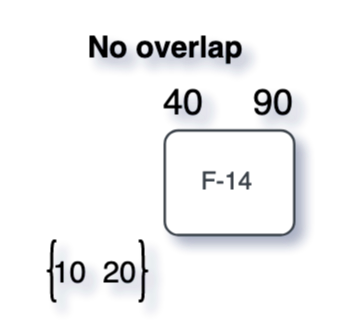
\includegraphics[scale=0.10]{Figures/No Overlap.png}
%     \caption{No Overlap between range-query and file}\label{fig:no_overlap}
% \end{figure}

% \begin{figure}
%     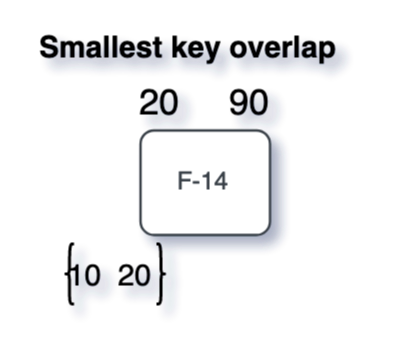
\includegraphics[scale=0.10]{Figures/Smallest Key Overlap.png}
%     \caption{Smallest (single) key overalp with range-query}\label{fig:smallest_key_overlap}
% \end{figure}

% \begin{figure}
%     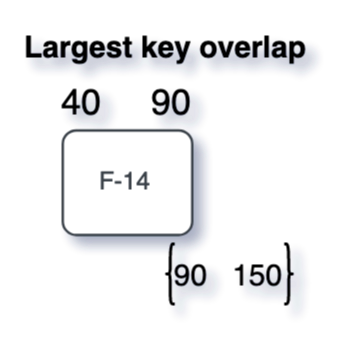
\includegraphics[scale=0.10]{Figures/Largest Key Overlap.png}
%     \caption{Largest (single) key overlap with range-query}\label{fig:largest_key_overlap}
% \end{figure}

% \begin{figure}
%     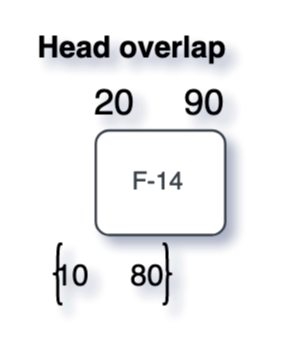
\includegraphics[scale=0.10]{Figures/Head Overlap.png}
%     \caption{Head (more than one key) overlap with range-query}\label{fig:head_overlap}
% \end{figure}

% \begin{figure}
%     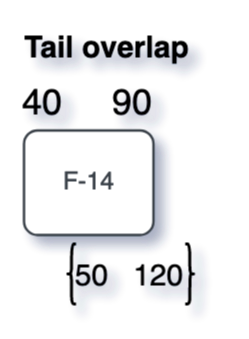
\includegraphics[scale=0.10]{Figures/Tail Overlap.png}
%     \caption{Tail (more than one key) overlap with range-query}\label{fig:tail_overlap}
% \end{figure}

% \begin{figure}
%     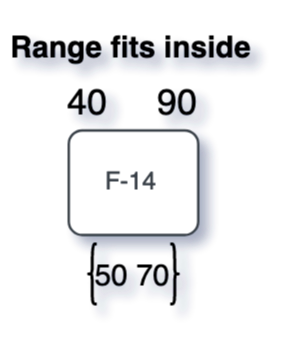
\includegraphics[scale=0.10]{Figures/Range Fits Overlap.png}
%     \caption{Range query overlap by file}\label{fig:range_fits_overlap}
% \end{figure}

% \begin{figure}
%     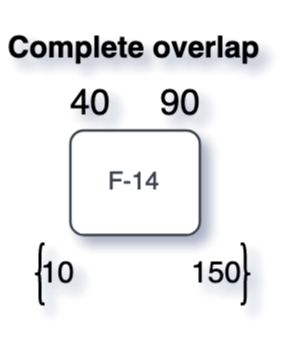
\includegraphics[scale=0.10]{Figures/Complete Overlap.png}
%     \caption{Complete file overlap}\label{fig:complete_overlap}
% \end{figure}
